\section{Computation architectures}
\label{sec:comparch}
Computations are often performed on a computer's Central Processing Unit - a CPU.
A CPU is often fastest for calculations and task not requiring immense computing power, as well as any calculation not parallelisable
The CPU consist of only a few cores which are highly optimized for sequential serial processing.\citep{whatisgpu}
In recent years developers and scientists seem to have developed an interest for performing calculations on Dedicated Graphic Processing Units.\citep{gpurise}
This is a different architecture which was intended for graphics processing
It seems that the GPU can be utilised for General Purpose GPU computing - GPGPU for some computational problems, with an performance improvement over a CPU.
In the following text we explore the possibilities that a GPU architecture offers.

GPUs are commonly used in the private and professional world, for computer gaming and accelerating graphic intensive programs such as Adobe Photoshop and 3D modelling tools. \citep{NVIDIAADOBE,STEAMHW}
Their architecture can also be used for advantageously for certain types of computations, primarily computations which can be done in parallel. 
An example of this can be calculating different properties of the pixels on a screen. 
The screen can then be divided into different sections called blocks and the computations for each block of data is divided internally on the GPU to its threads
This is possible because the specific calculations do not require results from the other calculations, IE. they are parallelisable.
Unlike the cores in the CPU the cores in the GPU are not optimized for sequential serial processing, instead its cores are designed to handle multiple tasks at once. 
As such running sequential code on the CPU will be more efficient, whereas more compute-intensive functions may be better suited for the GPU; given the computations can be parallelised.\citep{NvidiaGPGPU}
The before mentioned example with pixels can be viewed as a matrix being divided into blocks, so the same method of parallelised workflow can be applied for linear algebra especially many operations on matrices where the problem can be split to non dependent subproblems.

\begin{figure}[h!]
\centering
 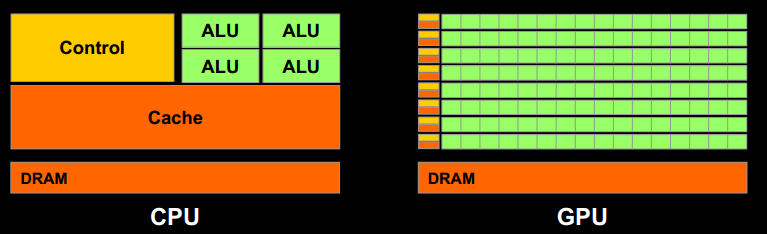
\includegraphics[width=1\textwidth]{figures/GPUCPUimage.png} % trim=4.85cm 15cm 0.85cm 1cm
\caption{A basic representation of the Transistor allocation on a GPU compared to a CPU}\label{image:GPUCPUimage}\citep{NvidiaCUDASeminar}
\vspace{-15pt}
\end{figure}

A simple representational comparison of a CPU - and a GPU's transistor usage is shown in \myref{image:GPUCPUimage}.
The GPU consists of more less powerful cores where as the CPU consists of fewer more powerful ones, the greater amount of cores allows for more computation power.
But to be able to utilise this computation power a problem must able to be split up, so many or all the cores in the GPU is used.
As of Q1 2015 an example of a modern high end desktop CPU is the Intel Haswell core i7 5960X which has 8 cores. \citep{puget}
A contemporary high end GPU is the NVIDIA GTX 980 which has 2048 CUDA cores. \citep{techpowerup,gtx980}
Due to their architectural differences the GPU allows for about 12 times more operations per second.

This makes the GPU particularly useful for large and complex computation, even some which are not graphical, if it is possibly to distribute the workload among the GPU cores.
However, the GPU has an overhead.
This means that moving data and computations to the GPU takes a lot af time.
Therefore the computation has to reach a certain size, before the advantage of parallel GPU computations exceeds the cost of transferring calculations onto the GPU.
To illustrate this problem as well as estimating an approximate computation size where the GPU is advantageous we have written some test problems. 
These problems perform different operations on all elements in a matrix. 

\subsection{GPU and CPU computations comparison}
To compare the computation speed of a GPU and CPU for operations on each element in a matrix we have written two programs.
A program written in regular C targeting the CPU and an equivalent program written in C with CUDA libraries targeting the GPU for computations.
Further explanation of this test and the full sourcecode of both programs and the accompanying scripts can be found in \myref{app:gpuoverhead} and \myref{app:cd}.

Both programs have been run with multiple sizes of the matrix.
The execution times for the two have then been compared to find an estimated threshold for when the GPU power overtakes the data transfer.
The test case for the following comparison consists of seven operations on a square matrix of size n.
The operations are division, multiplication, addition and subtraction.
The result can be seen on \myref{image:benchmark}.
\begin{figure}[h!]
\centering
 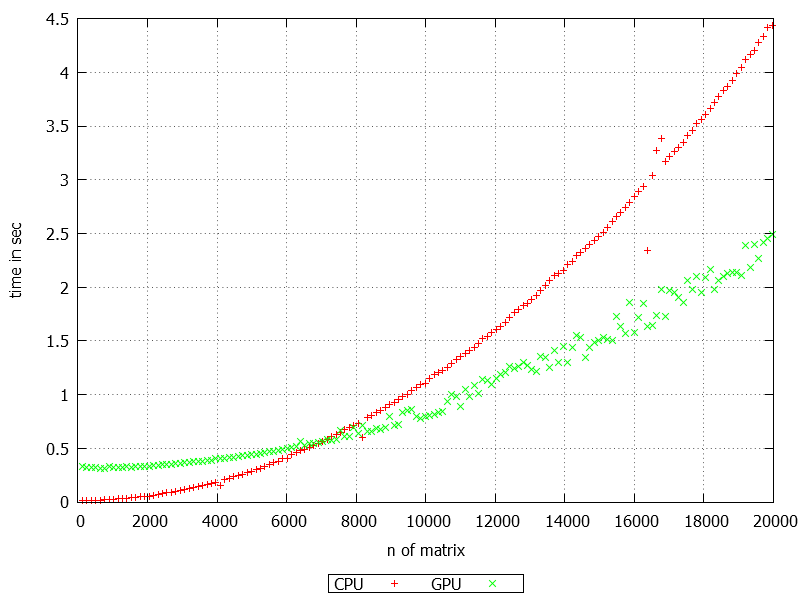
\includegraphics[width=1\textwidth]{figures/benchmark.png} % trim=4.85cm 15cm 0.85cm 1cm
\caption{A benchmark of performing seven operations on each element in a square matrix with size n on a CPU and a GPU respectively.}\label{image:benchmark}
\vspace{-15pt}
\end{figure}

The result show that in this case the GPU becomes advantageous when n reaches about 7000 as can be seen in \myref{image:benchmark}
When n is 7000 the size of the matrix represent operations on almost 50 millions elements.
This is a large amount of data but this is partly due to the simple operations done on the elements in the matrix, we believe that the threshold would happen earlier for a more complex operations in the elements in matrix.
\todo{Evt. lave et ny form for test som så er mere kompleks for at vise dette?}
In addition to the threshold, the result also confirms that as the dataset grows the GPU becomes exponentially more useful for computing the data fast.
